\documentclass{article}
\usepackage{ctex}
\usepackage{graphicx}
\usepackage{amsmath}
\usepackage{indentfirst}
\usepackage{titlesec}
\usepackage{setspace}
\usepackage{subfigure}
\usepackage{caption}
\usepackage{float}
\usepackage{booktabs}
\usepackage{geometry}
\usepackage{multirow}
\geometry{left=1.2cm,right=1.2cm,top=2cm,bottom=2cm}
\title{\songti \zihao{2}\bfseries HW4第8题Monte Carlo积分}
\titleformat*{\section}{\songti\zihao{4}\bfseries}
\titleformat*{\subsection}{\songti\zihao{5}\bfseries}
\renewcommand\thesection{\arabic{section}}
\author{王启骅 PB20020580}
\begin{document}
	\maketitle
	\section{题目}
用Monte Carlo方法计算如下定积分,并讨论有效数字位数。\\
1.$ \int_{0}^{5}\sqrt{x^2+2\sqrt{x}} $\\
2.$ \int_{0}^{7/10}dx\int_{0}^{4/7}dy\int_{0}^{9/10}dz\int_{0}^{2}du\int_{0}^{13/11}dv(5+x^2-y^2+3xy-z^2+u^3-v^3) $

	\section{算法原理}
第一题采用掷石法,由于被积函数f(x)在[0,5]单调递增,有最大值M=$ \sqrt{25+2\sqrt{5}} $,产生位于$ x\in [0,5],y\in [0,\sqrt{25+2\sqrt{5}}] $各n个均匀分布随机数,对于每一点,$ y<f(x) $则记录,满足的点数除以总点数并乘以区间面积即为积分结果。


第二题采用平均值方法,生成$ x\in [0,7/10],y\in [0,4/7],z\in [0,2],u\in[0,2],v\in[0,13/11] $的各n个均匀分布随机数
\begin{equation}
	\frac{1}{n}\sum_{i}^{n}g(x_i,y_i,z_i,u_i,v_i)
\end{equation}
为函数在区间内的均值,再乘以区间总体积得到积分值。
	\section{结果}
\begin{figure}[!h]
	\centering
	\subfigure[$ n=10^4 $]{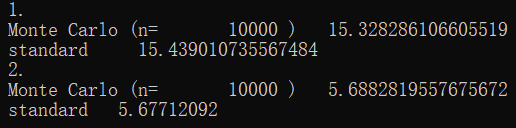
\includegraphics[scale=1]{n4}}
	\subfigure[$ n=10^5 $]{	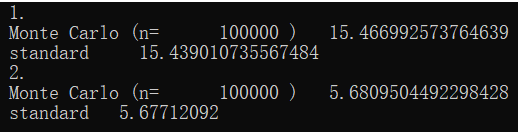
\includegraphics[scale=1]{n5}}
	\subfigure[$ n=10^6 $]{	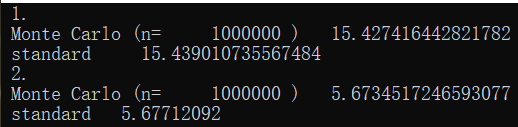
\includegraphics[scale=1]{n6}}
	\subfigure[$ n=10^7 $]{	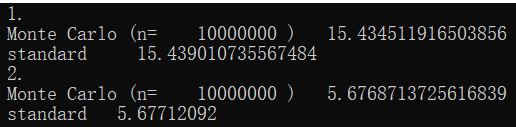
\includegraphics[scale=1]{n7}}
	\subfigure[$ n=10^8 $]{	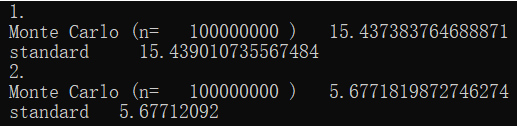
\includegraphics[scale=1]{n8}}
	\captionsetup{font={small},labelfont=bf}
	\caption{\heiti\zihao{-5}Monte Carlo积分结果}
	
\end{figure}
	如图1是积分结果与标准结果的对比,分别取$ n=10^4,10^5,10^6,10^7,10^8 $。对比得到在$ n=10^4 $,两题的积分有效位数都只有2位,$ n=10^5,10^6 $都有3位有效数字,$ n=10^7 $时第一题掷石法4位有效数字,第二题平均值法仍为3位有效数字,$ n=10^8 $第一题有4位有效数字,第二题5位有效数字
	\section{结论}
	有计算结果可得随着总点数n的量级增大,积分结果的精度有效数字增多,但当n较大是有效位数的增加并不明显,精度变化较慢。并且实验得到在相同总点数n的情况下的计算结果有效数字位数并不是每次都完全一致,具有一定的随机性。
\end{document}